\documentclass[11pt,a4paper,twoside,openright,titlepage,
                           headinclude,footinclude,BCOR5mm,
                           numbers=noenddot,cleardoublepage=empty,
                           tablecaptionabove]{scrbook}
\usepackage[T1]{fontenc}
\usepackage[utf8]{inputenc}
\usepackage[italian]{babel}
\usepackage[eulerchapternumbers,beramono, pdfspacing]{classicthesis}
\usepackage{arsclassica}
\usepackage{graphicx}
\usepackage{caption}
\usepackage{subfig}
\usepackage{amsmath}
\usepackage{amsthm}
\usepackage{listings}
\definecolor{mio_colore}{RGB}{242,243,244}
\definecolor{dkgreen}{rgb}{0,0.6,0}
\definecolor{gray}{rgb}{0.5,0.5,0.5}
\lstset{language=Matlab,basicstyle=\small\ttfamily,showstringspaces=false,numberstyle=\tiny\color{gray}, keywordstyle=\color{blue},commentstyle=\color{dkgreen},stringstyle=\color{red}, backgroundcolor=\color{mio_colore}}

\begin{document}

%@@@@@@@@@@@@@@@@@@@FRONT MATTER@@@@@@@@@@@@@@@@@@@@@@@@@@

\frontmatter

%------------------------------------------------------COPERTINA---------------------------------------------------
\title{Laboratorio Sperimentale di Matematica Computazionale 2016-2017}
\subtitle{Parte I}
\author{Paolo Giordano}
\maketitle

%------------------------------------------------------INDICE------------------------------------------------------

\tableofcontents

%@@@@@@@@@@@@@@@@@@@FRONT MATTER@@@@@@@@@@@@@@@@@@@@@@@@@@
\mainmatter

%PRIMO CAPITOLO
\chapter{Lezione II, 3 Marzo 2017}
\section{Esercizio 1}
La funzione \emph{graph\_laplacian} è:
\begin{lstlisting}[frame=trBL]
function L=graph_laplacian(A)
%A e' la matrice di adiacenza di un grafo non orientato
%L e' la matrice Laplaciana del grafo descritto da A
d=size(A);
a=ones(d(1),1);
L=spdiags(A*a,0,d(1),d(1))-A;
\end{lstlisting}

\subsection{\textbf{Punto a}}
Moltiplicando la matrice $L$ per il vettore $(1,1,\dots,1)^T$ si ottiene il vettore nullo, che ha di conseguenza norma nulla; infatti, dando il comando
\begin{lstlisting}[frame=lines]
>> norm(L*ones(60,1))
\end{lstlisting}
si ottiene
\begin{lstlisting}[frame=lines]
ans=

         0
\end{lstlisting}
Sia 
\[
A=
\begin{pmatrix}
a_{11} & a_{12} & \dots \\
a_{21} & a_{22} & \dots \\
\vdots & \vdots & \ddots
\end{pmatrix}
\]
Per dimostrare che $(1,1,\dots,1)^T$ è autovettore del Laplaciano qualunque sia il grafo $\mathcal{G}$, è sufficiente scrivere $L$ come 
\[
L=D-A=
\begin{pmatrix}
\displaystyle\sum_{\substack{i=1 \\ j \ne 1}} a_{ij} & -a_{12} & -a_{13} & \dots \\
-a_{21} & \displaystyle\sum_{\substack{i=2 \\ j \ne 2}} a_{ij} & -a_{23} & \dots \\
-a_{31} & -a_{32} & \displaystyle\sum_{\substack{i=3 \\ j \ne 3}} a_{ij} & \dots \\
\vdots  & \vdots & \vdots & \ddots
\end{pmatrix}
\] 
e moltiplicare questa matrice per $(1,1,\dots,1)^T$, in questa maniera si ottiene un vettore che ha componente $k-esima$ uguale a 
\[
\displaystyle\sum_{\substack{i=k \\ j \ne k}} a_{ij} + \displaystyle\sum_{\substack{i=k \\ j \ne k}} -a_{ij},
\]
che è uguale a zero per ogni k.

\subsection{\textbf{Punto b}}

La matrice $L$ è simmetrica poichè si ottiene sottraendo ad una matrice diagonale una matrice simmetrica ($L=D-A$).
Per verificare che i suoi autovalori siano tutti maggiori o uguali di zero, si può usare la funzione $eigs$ nel modo seguente:
\begin{lstlisting}[frame=lines]
>> eigs(L,2,'SM')
\end{lstlisting}
il quale ci dice che i due autovalori più piccoli sono: 
\begin{lstlisting}[frame=lines]
ans =

   1.61624894705837e-01
  -2.22044604925031e-17

\end{lstlisting}
%$ans$ è positivo, ed essendo il più piccolo autovalore ci assicura che tutti gli altri autovalori siano maggiori di zero.
$ans$ è formato da due elementi: il primo maggiore di zero e l'altro minore della precisione di macchina e per questo approssimabile a zero.
Essendo questi i due autovalori più piccoli, siamo sicuri che tutti gli altri siano maggiori di zero.
\par
È possibile dimostrare che questa è una proprietà generale della matrice Laplaciana, infatti, applicando il primo teorema di Gerschgorin alla matrice L, si osserva che i cerchi di Gerschgorin hanno tutti centro positivo e raggio uguale alla distanza del centro dall'origine degli assi. (I centri dei cerchi sono tutti positivi perchè gli elementi sulla diagonale di L sono somme di elementi della matrice A, che è composta da soli 0 e 1.)

\subsection{\textbf{Punto c}}

Diamo il comando
\begin{lstlisting}[frame=lines]
>> eigs(L,2,'SM')
\end{lstlisting}
il quale da come risposta
\begin{lstlisting}[frame=lines]
ans=

         0.243401746139933
         0.000000000000000
\end{lstlisting}
da cui si ottiene che il secondo autovalore più piccolo di L è 
\[
\lambda_{2}=0.243401746139933
\]


\section{Esercizio 2}
La funzione \emph{Fiedler\_vector} è:
\begin{lstlisting}[frame=trBL]
function [l,x,perm]=Fiedler_vector(A)
% A matrice di Adiacenza di un grafo
% x e' il vettore di Fiedler
% l e' il secondo autovalore piu' piccolo di L
% perm e' la permutazione che ordina x in ordine crescente

L=graph_laplacian(A); %Calcolo il Laplaciano di A 
[V,D]=eigs(L,2,'SM');    %Calcolo autovalore
                         %ed autovettore di Fiedler
l=D(1,1);
x=V(:,1);
[y,perm]=sort(x);     %Calcolo la permutazione che ordina x
B=A(perm, perm);      %Riordino A in base alla permutazione perm
spy(B);                  %Visualizziamo la struttura 
                         %della matrice B
[C,d]=spdiags(B);     %Calcolo l'ampiezza di banda di B e di A
band_temp=size(d);
band1=band_temp(1);
[C,d]=spdiags(A);
band_temp=size(d);
band2=band_temp(1);
if band1<band2    %Verifico se la banda di B 
                   %e' minore di quella di A
    disp('La banda di B e' minore di quella di A.')
end
\end{lstlisting}
Per il calcolo del Laplaciano di A si è usata la funzione \emph{graph\_laplacian} dell'esercizio 1.\\
Tramite la funzione \emph{spdiags} otteniamo un vettore \emph{d} che ha dimensione pari al numero di diagonali non nulle di una matrice sparsa, ovvero il suo numero di banda.

\begin{figure}[h!]
\begin{center}
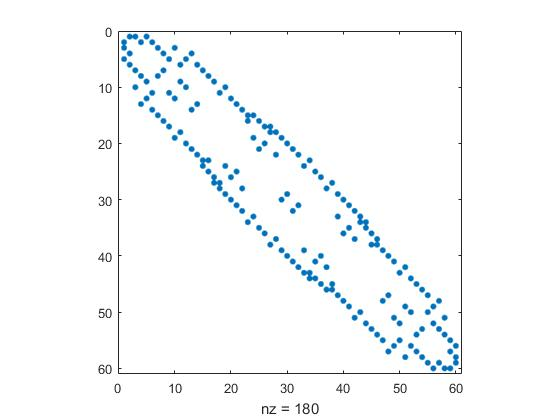
\includegraphics[width=0.6\textwidth]{figs/SpyB.jpg}
\caption{Grafico della struttura della matrice $B$, ottenuto con la funzione \emph{spy}.}
\end{center}
\end{figure}

\newpage
\section{Esercizio 3}
\subsection{\textbf{Punto a}}
La funzione \emph{incidence\_matrix} è:
\begin{lstlisting}[frame=trBL]
function M=incidence_matrix(A)
% A matrice di adiacenza di un grafo
% M sua matrice di incidenza

%Le diagonali le rendo uguali a zero
%Controlliamo se A e' simmetrica
if A==A'
    %Se A e' simmetrica consideriamo la sua triangolare superiore
    A1=triu(A)-diag(diag(A)); 
    %numero di elementi di A1 non nulli
    d=size(A);
    count=nnz(A1);
    M=zeros(d(1),count);
    column=1;
    %Creo la matrice M
    for k=1:d(1)
        for j=k:d(1)
            if A1(k,j)~=0
                M(k,column)=1;
                M(j,column)=-1;
                column=column+1;
            end
        end
    end
else
    %Se A non e' simmetrica la considero tutta
    A1=A-diag(diag(A));
    d=size(A);
    count=nnz(A1);
    M=zeros(d(1),count);
    column=1;
    %Creo la matrice M
    for k=1:d(1)
        for j=1:d(1)
            if A1(k,j)~=0
                M(k,column)=1;
                M(j,column)=-1;
                column=column+1;
            end
        end
    end
end
\end{lstlisting}

\subsection{\textbf{Punto b}}
Assegniamo la matrice \emph{bucky} ad \emph{A}:
\begin{lstlisting}[frame=lines]
>>[A,v]=bucky;
\end{lstlisting}
Calcoliamo la Laplaciana di A:
\begin{lstlisting}[frame=lines]
>>L=graph_laplacian(A);
\end{lstlisting}
Verifichiamo che si ha $L=M*M^T$:
\begin{lstlisting}[frame=lines]
>>M=incidence_matrix(A);
>>if L==M*M'
         disp('L=M*M^T')
     end
\end{lstlisting}
L'output è:
\begin{lstlisting}[frame=lines]
L=M*M^T
\end{lstlisting}
Osserviamo inoltre che
\begin{lstlisting}[frame=lines]
>> size(M)

ans=
 
        60     60
>> rank(M)

ans=

         59
\end{lstlisting}
cioè che \emph{rank(M)=n-1}.
\newpage
\section{Esercizio 4}
La funzione \emph{solve\_augmented} è:
\begin{lstlisting}[frame=trBL]
function [x]=solve_augmented(M,b)
    % USO: x=solve_augmented(M, b),
    % M matrice di incidenza di un grafo,
    % b vettore dei termini noti del sistema lineare Lx=b
    [n,m]=size(M);
    B=sparse([eye(m) M';M zeros(n)]); %B deve essere sparsa
    [Q,R,P]=qr(B); %utilizziamo il metodo qr con pivot sulle
    % colonne per calcolare una fattorizzazione
    % "rank-revealing" cioe' dove le ultime t righe di R sono 
    %nulle se rank(R)=n-t;
    c1=rand(m,1);
    c2=M*c1-b;
    c=[c1;c2];
    z=Q\c; %soluzione del sistema Qz=c
    soglia=0.0000000001;
    r=sum(abs(diag(R))>soglia); % rango di R
    if abs(z(r+1:n+m))>10^-12*norm(z) || r==n+m
    %controlla che z(r+1:n+m)==0 e che R sia singolare
    error('qualcosa va male, vettore b non adeguato?');
    end
    R1=R(1:r,1:r); %minore principale di testa di R di rango pieno
    z1=z(1:r);
    V1=R(1:r,r+1:end); %prime r righe delle ultime colonne 
                       %della matrice R
    alpha=ones(1,n+m-r); % vettore qualsiasi di 
                         %dimensioni opportune...
    w1=R1\(z1-V1*alpha);
    w=[w1;alpha];
    y=P*w; % occorre permutare le componenti di w
    x=y(m+1:end);
    % verifica che x sia soluzione di Lx=b
end
\end{lstlisting}
\newpage
\section{Test delle Funzioni}
Test delle funzioni tramite \emph{testL2}:
\begin{lstlisting}[frame=lines]
>>testL2
Laplacian test passed
Incidence matrix test passed
La banda di B e' minore di quella di A.
Fiedler test passed
Augmented solution test passed
\end{lstlisting}
Dove l'output \emph{"La banda di B è minore di quella di A."} è dovuto all'esecuzione della funzione \emph{incidence\_matrix}, la quale inoltre restituisce, tramite funzione \emph{spy}, il seguente grafico:
\begin{figure}[h]
\begin{center}
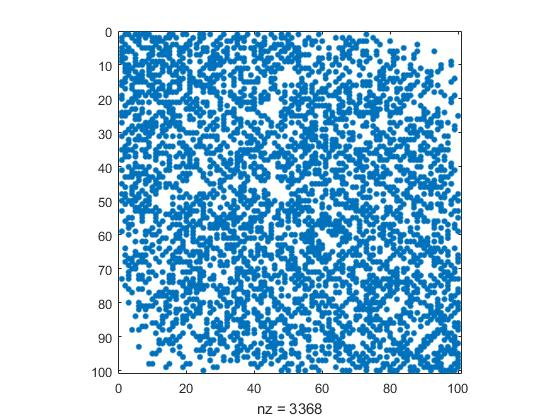
\includegraphics[width=\textwidth]{figs/testL2fig.jpg}
\caption{Output di \emph{spy} della funzione \emph{incidence\_matrix} durante il \emph{testL2}.}
\end{center}
\end{figure}

\chapter{Lezione III, 8 Marzo 2017}
\section{Esercizio 1}
La funzione \emph{mean\_classifier} è:
\begin{lstlisting}[frame=trBL]
function [class]=mean_classifier(TrainingSet,DigitsTraining...
   ,TestSet)
% TrainingSet: una matrice mxn contente m immagini su n vettori
% DigitsTraining: vettore di n componenti che riporta la cifra
% rappresentata di ogni immagine in TraininSet
% TestSet: matrice di immagini da classificare
% class: vettore che conterra' la 
%classificazione delle cifre nel TestSet
M=zeros(256,10);
cont=zeros(1,10);
%leggiamo le occorrenze nel vettore DigitsTraining 
%e creiamo la matrice M
for i=1:1707
    cont(DigitsTraining(i)+1)=cont(DigitsTraining(i)+1)+1;
    M(:,DigitsTraining(i)+1)=M(:,DigitsTraining(i)+1)+...
         TrainingSet(:,i);
end
for i=1:10
    M(:,i)=M(:,i)/cont(i);
end
%mostriamo a schermo le immagini delle colonne di M
for c=1:10
     subplot(2, 5, c)
     ima2(M(:, c))
end
%classifichiamo le cifre di TestSet tramite le medie 
%contenute nella matrice M
for i=1:2007
    v=zeros(1,10);
    for k=1:10
        v(k)=norm(TestSet(:,i)-M(:,k));
    end
    for j=1:10
        if v(j)==min(v)
            class(i)=j-1;
        end
    end
end
\end{lstlisting}

Salviamo nel vettore \emph{class} la classificazione delle cifre nel TestSet:
\begin{lstlisting}[frame=lines]
>>load dataset_digits
>>[class]=mean_classifier(TrainingSet, DigitsTraining, TestSet)
\end{lstlisting}
L'output della funzione \emph{ima2} è:
\begin{figure}[h!]
\begin{center}
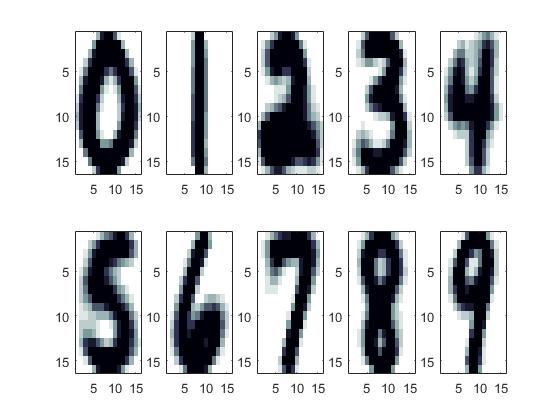
\includegraphics[width=\textwidth]{figs/ima2.jpg}
\caption{Immagini medie salvate nelle colonne di M.}
\end{center}
\end{figure}

Per vedere quanto è vicino il vettore \emph{class} alla reale classificazione delle cifre di TestSet, lanciamo il seguente programma:
\begin{lstlisting}[frame=trBL]
function precision_test(class, DigitsTest)
cont=0;
for i=1:2007
    if class(i)==DigitsTest(i)
        cont=cont+1;
    end
end
precisione=(cont/2007)*100
\end{lstlisting}
La sua esecuzione restituisce una precisione dell'$80\%$ circa.
\begin{lstlisting}[frame=lines]
>>precision_test(class, DigitsTest)

precisione=

       80.8670
\end{lstlisting}
\newpage
\section{Esercizio 2}
La funzione \emph{svd\_classifier} è:
\begin{lstlisting}[frame=trBL]
function [class]=svd_classifier(TrainingSet, DigitsTraining,...
    TestSet, h)
% TrainingSet: m immagini vettorizzate su n componenti
% DigitsTraining: vettore di m componenti che 
% riporta la cifra rappresentata
% di ogni immagine in TraininSet
% TestSet: matrice di immagini da classificare
% h :intero
% class: vettore contente la classificazione delle 
% cifre nel TestSet

%contatore occorrenze di ogni cifra
cont=zeros(1,10);
for i=1:1707
    cont(DigitsTraining(i)+1)=cont(DigitsTraining(i)+1)+1;
end
%ordiniamo la matrice TrainingSet in base all'ordine di DigitsTest
[n,m]=size(TrainingSet);
M=TrainingSet';
M(:,n+1)=DigitsTraining;
B=sortrows(M,n+1);
B(:,end)=[];
M=B';
%calcolo dell'SVD degli A_i, plot degli U_i
%creazione matrice BigU
x=0;
y=cont(1);
BigU=zeros(256,10*h);
for i=1:10
    [U,S,V]=svd(M(:,x+1:y));
    if i<10
        x=y;
        y=y+cont(i+1);
    end
    subplot(2, 5, i)
    ima2(U(:,1))
    BigU(:,(i-1)*h+1:i*h)=U(:,1:h);
end

v=zeros(1,10);
for i=1:2007
    for k=1:10
        v(k)=norm(((eye(256)-(BigU(:,(k-1)*h+1:k*h))...
            *(BigU(:,(k-1)*h+1:k*h))')*TestSet(:,i)));  
    end
    for k=1:10
        if v(k)==min(v)
            class(i)=k-1;
        end
    end
    v=zeros(1,10);
end
end    
\end{lstlisting}

\emph{svd\_classifier} restituisce la seguente immagine:
\begin{figure}[h!]
\begin{center}
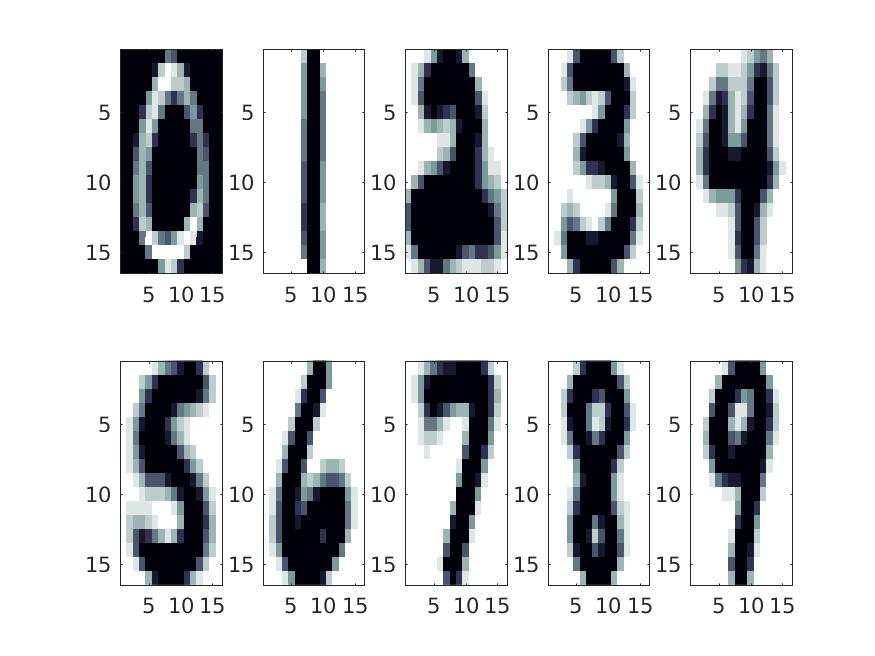
\includegraphics[width=\textwidth]{figs/svd_classifier.jpg}
\caption{Immagini ottenute dal classificatore SVD.}
\end{center}
\end{figure}
\par
La percentuale di immagini test salvate correttamente la calcoliamo con la function \emph{percent\_esatti}:
\begin{lstlisting}[frame=trBL]
function percent_esatti(DigitsTest,DigitsTraining,TestSet,...
    TrainingSet)
percentuale=zeros(1,16);
a=1;
for h=5:20
    y=svd_classifier2(TrainingSet,DigitsTraining,TestSet,h)-...
        DigitsTest;
    esatti=2007-nnz(y);
    percentuale(a)=esatti/2007*100;
    a=a+1;
end
axis('equal')
plot([5:20],percentuale, '*b')
\end{lstlisting}
dove la funzione \emph{svd\_classifier2} è la funzione \emph{svd\_classifier} che non plotta i primi vettori singolari sinistri di U. L'immagine che si ottiene è:
\begin{figure}[h!]
\begin{center}
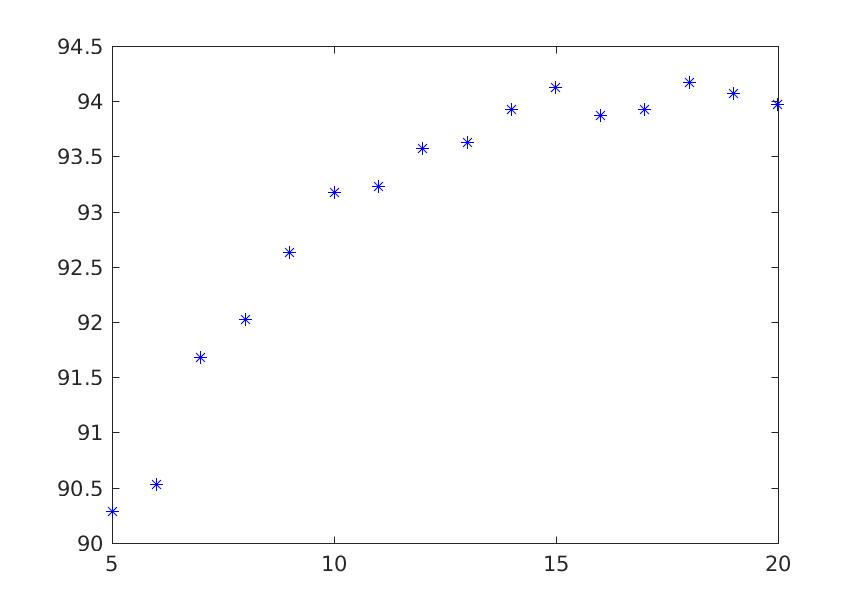
\includegraphics[width=\textwidth]{figs/percentuale_esatti.jpg}
\caption{Percentuale di vettori classificati correttamente.}
\end{center}
\end{figure}
\newpage
Per vedere se tutte le cifre vengono classificate con la stessa difficoltà lanciamo la function \emph{percent\_cifre}:
\begin{lstlisting}[frame=trBL]
function percent_cifre(DigitsTest, DigitsTraining, TestSet,...
    TrainingSet)
%contatore occorrenze di ogni cifra
    cont=zeros(1,10);
    for i=1:2007
        cont(DigitsTest(i)+1)=cont(DigitsTest(i)+1)+1;
    end
%plot della percentuale di precisione per ogni cifra e per ogni
%h tra 5 e 20
for h=5:20
    percentuale=zeros(1,10);
    [class]=svd_classifier2(TrainingSet, DigitsTraining,...
        TestSet, h);
    for i=1:2007
        if class(i)==DigitsTest(i)
        percentuale(DigitsTest(i)+1)=...
            percentuale(DigitsTest(i)+1)+1;
        end
    end
    for k=1:10
        percentuale(k)=percentuale(k)/cont(k);
    end
    subplot(4,4,h-4)
    plot(0:9,percentuale,'*b')
    title(h)
end
\end{lstlisting}
\par
che restituisce la seguente immagine:

\begin{figure}[h!]
\begin{center}
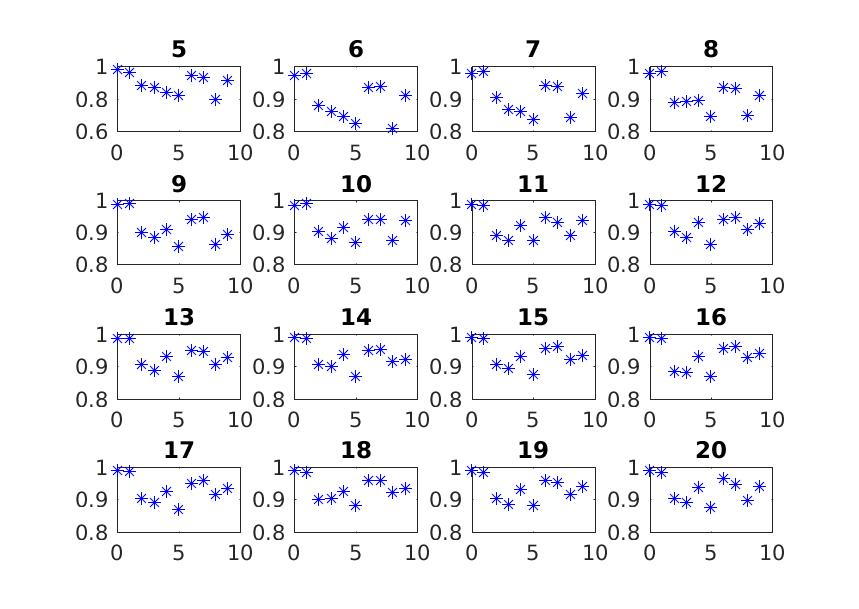
\includegraphics[width=\textwidth]{figs/percent_cifre.jpg}
\caption{Percentuale di cifre esatte per ogni cifra e per ogni h tra 5 e 20.}
\end{center}
\end{figure}

Dall'immagine si evince che non tutti i numeri presentano la stessa difficoltà ad essere riconosciuti, infatti il 5 viene riconosciuto con percentuale molto minore dello 0.\\
Se ad esempio proviamo ad utilizzare un numero diverso di vettori singolari per rappresentare la cifra 5, osserviamo che la sua precizione cala. La seguente immagine mostra la precisione che si ottiene impostando a 4 il numero di vettori singolari del 5:

\begin{figure}[b!]
\begin{center}
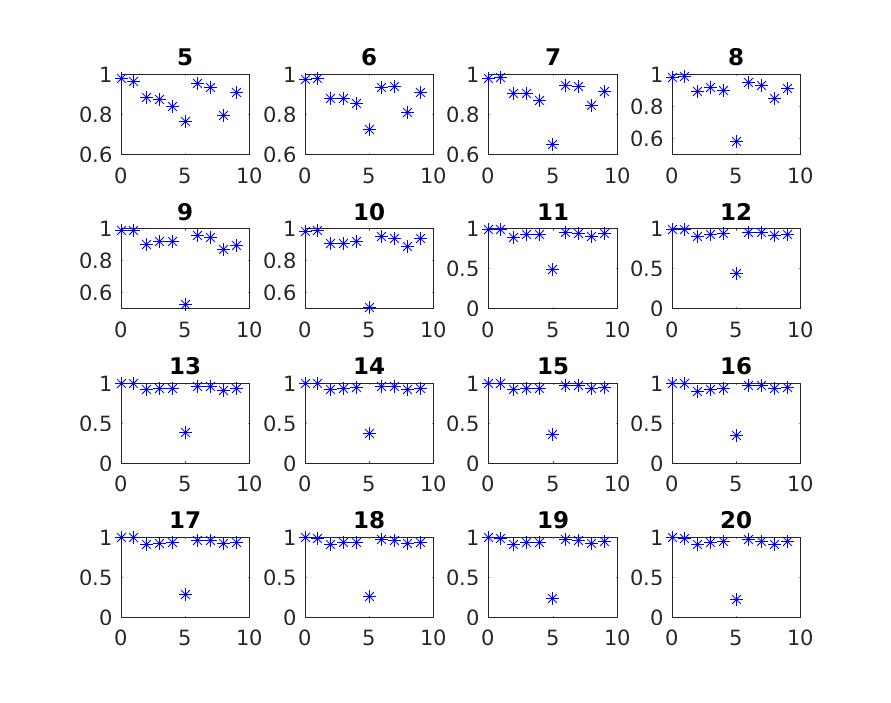
\includegraphics[width=0.7\textwidth]{figs/percent_cifre2.jpg}
\caption{Numero di vettori singolari del 5=4.}
\end{center}
\end{figure}
\newpage
\section{Test delle funzioni}
Testiamo le funzioni tramite la funzione \emph{test\_L3}:
\begin{lstlisting}[frame=lines]
>>testL3
Test frequenza passed
Test frequenza svd passed
Test frequenza svd passed
Test frequenza svd passed
Test frequenza svd passed
Test frequenza svd passed
\end{lstlisting}

\chapter{Lezione IV, 10 Marzo 2017}
\section{Esercizio 1}
La funzione \emph{cos\_vector} è:
\begin{lstlisting}[frame=trBL]
function vc=cos_vector(A, q)
% A: matrice termini-documenti
% q: vettore di query
% vc: vettore, vc(j) memorizza il coseno dell'angolo
% tra la colonna a_j e il vettore q

[m,n]=size(A);
vc=zeros(1,n);
for i=1:n
    vc(i)=(A(:,i)'*q)/(norm(q)*norm(A(:,i)));
end
\end{lstlisting}
\section{Esercizio 2}
La funzione \emph{precision\_recall} è:
\begin{lstlisting}[frame=trBL]
function [P, R]=precision_recall(vc, query_index, epsilon, M)
% vc vettore dei coseni
% epsilon: threshold
% query_idx: indice di una query in Q_med
% M: matrice che associa ad ogni query_index la lista 
% dei documenti rilevanti
% P: valore di Precision
% R: valore di Recall

[n,m]=size(vc);
pos=zeros(m);
Dt=0;
Dr=0;
Nr=sum(M(query_index,:));

for i=1:m
    if vc(i)>epsilon
        Dt=Dt+1;
        pos(i)=1;
    end
end
a=find(pos);
b=find(M(query_index,:));
inter=intersect(a,b);
Dr=length(inter);
P=Dr/Dt;
R=Dr/Nr;
Dr
Dt
Nr
end
\end{lstlisting}
Testiamo la funzione:
\begin{lstlisting}[frame=lines]
>>x=523677;
>>query_index=mod(x,30)+1;
>>vc=cos_vector(A_med, Q_med(:,query_index));
>>epsilon=0.01;
>>[P, R]=precision_recall(vc, query_index, epsilon, Med_rel)

P=

    0.1111
    
R=

    0.9744
\end{lstlisting}

Per ottenere il grafico delle medie di precision e recall lanciamo lo script \emph{media\_prec}:
\begin{lstlisting}[frame=trBL]
function media_prec(A,Q,M)
% A,Q,M sono A_med, Q_med, Med_rel
PM=zeros(1,10); %vettori delle medie
RM=zeros(1,10);
k=1;
for j=0.01:0.01:0.1
    Pm=0;
    Rm=0;
    for i=1:30
        vc=cos_vector(A,Q(:,i));
        [P, R]=precision_recall(vc, i, j, M);
        Pm=Pm+P;
        Rm=Rm+R;
    end
    PM(k)=Pm/30; %calcolo della media
    RM(k)=Rm/30;
    k=k+1;
end
a=0.01:0.01:0.1;
plot(a,PM,'or')
hold on
plot(a,RM,'ob')
\end{lstlisting}
Da questa funzione si ottiene il seguente grafico:

\begin{figure}[h!]
\begin{center}
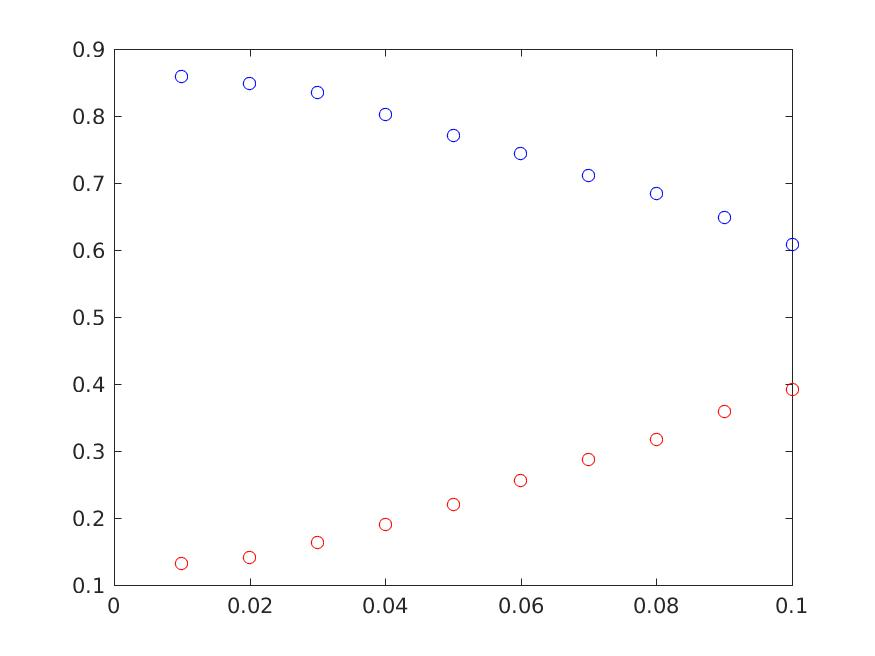
\includegraphics[width=\textwidth]{figs/media_prec.jpg}
\caption{Medie di precision e recall, con precision rossa e recall blu.}
\end{center}
\end{figure}
\newpage
\section{Esercizio 3}
La funzione \emph{LSI} è:
\begin{lstlisting}[frame=trBL]
function [vc]=LSI(A, q, k)
% A: matrice terminixdocumenti
% q: vettore query
% k: intero
% vc: vettore dei coseni

[n,m]=size(A);
for j=1:m
    A(:,j)=A(:,j)/norm(A(:,j));
end
[U,S,V]=svds(A,k);
C=V*(S');
vc=zeros(1,k);
for j=1:k
    vc(j)=(C(j,:)*(U'*q))/(norm(C(j,:))*norm(U'*q));
end
\end{lstlisting}
Per controllare le medie con valori di k=25,50,75,100 usiamo lo script \emph{media\_LSI}:
\begin{lstlisting}[frame=trBL]
function media_LSI(A,Q,M)
PM=zeros(1,4);
RM=zeros(1,4);
epsilon=0.01;
j=1;
for k=25:25:100
    Pm=0;
    Rm=0;
    for i=1:30
        vc=LSI(A, Q(:,i), k);
        [P, R]=precision_recall(vc, i, epsilon, M);
        Pm=Pm+P;
        Rm=Rm+R;
    end
    PM(j)=Pm/30;
    RM(j)=Rm/30;
    j=j+1;
end
x=25:25:100;
plot(x,PM,'or')
hold on
plot(x,RM,'ob')
\end{lstlisting}
Questa function ci restituisce il seguente grafico:
\begin{figure}[h!]
\begin{center}
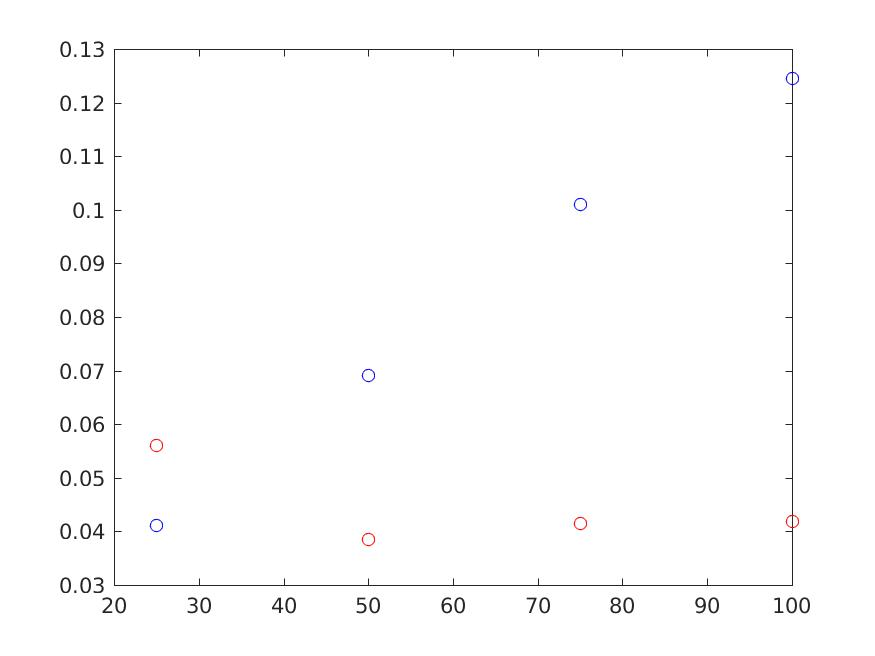
\includegraphics[width=\textwidth]{figs/media_LSI.jpg}
\caption{Medie di precision e recall, con precision rossa e recall blu.}
\end{center}
\end{figure}

%#################################   DA QUI ###############################################################

\chapter{Lezione V, 15 Marzo 2017}
\section{Esercizio 1}
La funzione \emph{build\_matrix} è:
\begin{lstlisting}[frame=trBL]
function Phat=build_matrix(A, alpha)
% A: matrice di adiacenza di un grafo
% alpha: parametro di "teletrasporto" valore tipico 0.15
% Phat=(1-alpha)*Pbar+\alpha evT

[n,m]=size(A);
e=ones(n,1);
d=zeros(n,1);
v=e/n;
outdegree=A*ones(m, 1);
for i=1:n
    if outdegree(i)==0
        P(i,:)=A(i,:);
    else
        P(i, :)=A(i, :)/outdegree(i);
    end
end
for i=1:n
    if outdegree(i)==0
        d(i)=1;
    else
        d(i)=0;
    end
end
Pbar=P+d*v';
Phat=(1-alpha)*Pbar+alpha*e*v';
\end{lstlisting}
\section{Esercizio 2}
La funzione \emph{pagerank} è:
\begin{lstlisting}[frame=trBL]
function [pr]=pagerank(A, alpha)
% A: matrice di adiacenza di un grafo
% alpha: parametro di teletrasporto valore tipico 0.15
% pr: vettore di pageRank costruito come l'autovettore sinistro
% di Phat relativo a lambda=1
Phat=build_matrix(A, alpha);
[V,D]=eigs(Phat',1);
pr=V';
\end{lstlisting}
Per fare il plot delle componenti vettore di PageRank usiamo lo script \emph{pageplot}:
\begin{lstlisting}[frame=trBL]
function pageplot(A)
hold on
alpha=[0.15, 0.1, 0.01, 10^-8, 10^-12];
plot(pagerank(A,alpha(1)),'y');
plot(pagerank(A,alpha(2)),'m');
plot(pagerank(A,alpha(3)),'c');
plot(pagerank(A,alpha(4)),'r');
plot(pagerank(A,alpha(5)),'g');
\end{lstlisting}

\begin{figure}[h!]
\begin{center}
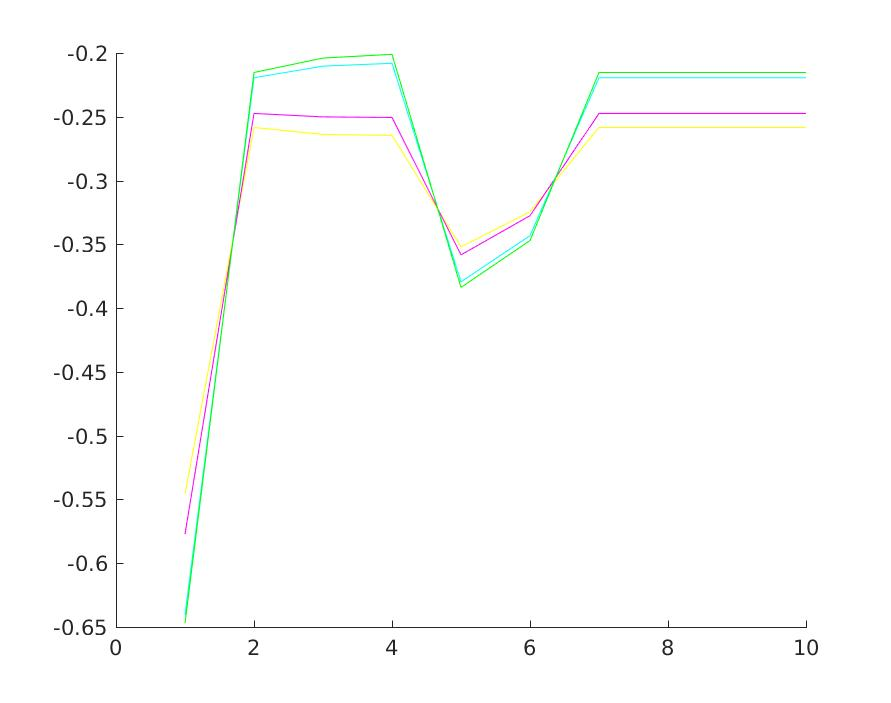
\includegraphics[width=\textwidth]{figs/pageplot.jpg}
\caption{Grafico componenti PageRank.}
\end{center}
\end{figure}

\newpage
\section{Esercizio 3}
La funzione \emph{P\_times\_x} è:
\begin{lstlisting}[frame=trBL]
function [y]=P_times_x(P, x, alpha)
% P: matrice ottenuta dalla matrice di adiacenza
% scalando le righe per l'outdegree
% alpha: parametro di teletrasporto
% x: vettore
[m,n]=size(P);
e=ones(n,1);
v=e/n;
y=(1-alpha)*P'*x;
gamma = 1-norm(y,1);
y=y+gamma*v;
end
\end{lstlisting}

\section{Esercizio 4}
\subsection{\textbf{Parte 1}}
La funzione \emph{pr\_powermethod} è:
\begin{lstlisting}[frame=trBL]
function [pr]=pr_powermethod(A, alpha)
% A: matrice di adiacenza di un grafo
% alpha: parametro di teletrasporto
% pr: vettore di PageRank
[n,m]=size(A);
somma = sum(A, 2);
B = find(somma==0);
somma(B) = 1;
C = spdiags(1./somma, 0, n, n);
D = C*A;

i = 1;
pr = rand(n, 1);
pr = pr/norm(pr, 1);
p = zeros(n, 1);
while((i<100) && (norm(pr-p)>10^(-7)))
    p = pr;
    pr = P_times_x(D, pr, alpha);
    error(i) = norm(pr-p);
    i = i+1;
end

plot(error,'b')

end
\end{lstlisting}
Questa funzione traccia anche il grafico degli errori. Usandola sulla matrice \emph{stanford\_web} otteniamo il seguente grafico:
\begin{figure}[h!]
\begin{center}
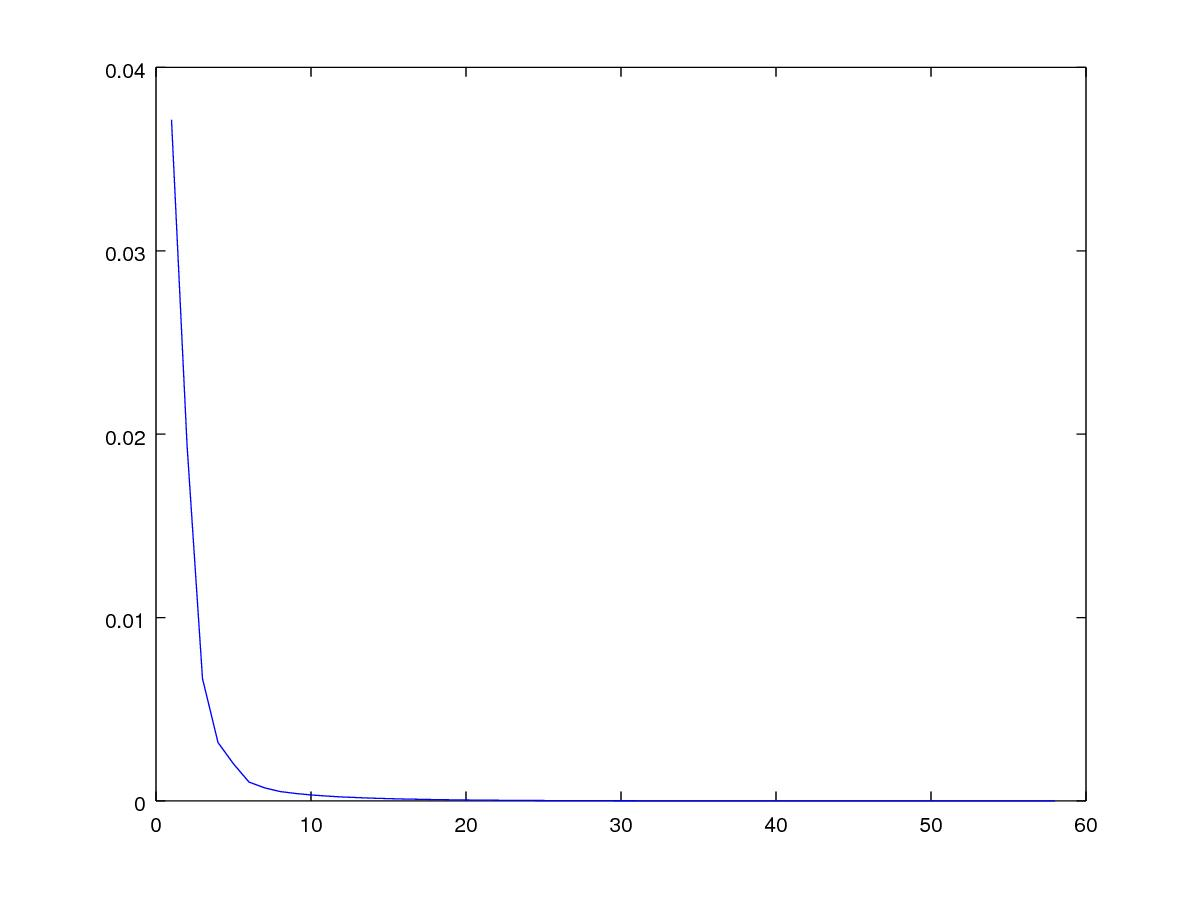
\includegraphics[width=\textwidth]{figs/pr_powermethod.jpg}
\caption{Grafico errori di pr\_powermethod.}
\end{center}
\end{figure}

\newpage
\subsection{\textbf{Parte 2}}
Creiamo la funzione \emph{P\_times\_x\_norm}:
\begin{lstlisting}[frame=trBL]
function y = P_times_x_norm(A, x, alpha)

y = norm(x, 1)*P_times_x(A, x/norm(x, 1), alpha);

end
\end{lstlisting}
La funzione \emph{pagerank\_eigs} è:
\begin{lstlisting}[frame=trBL]
function [pr]=pagerank_eigs(A,alpha)

[n,m]=size(A);
somma = sum(A, 2);
B = find(somma==0);
somma(B) = 1;
C = spdiags(1./somma, 0, n, n);
D = C*A;

y=@(x) P_times_x_norm(D, x, alpha);
[V,D]=eigs(y, n, 1);
pr=V;

\end{lstlisting}

\subsection{\textbf{Parte 3}}

Usiamo la funzione \emph{pr\_powermethod\_2} che si ottiene dalla funzione
\emph{pr\_powermethod} semplicemente cancellando l'istruzione di \emph{plot}.
Per confrontare la velocità di convergenza dei due metodi usiamo lo script \emph{confronto\_tempi}:
\begin{lstlisting}[frame=trBL]
function confronto_tempi(A)

disp('powermethod con alpha=0.15')
tic;
a=pr_powermethod_2(A,0.15);
toc;

disp('pagerank_eigs con alpha=0.15')
tic;
b=pagerank_eigs(A,0.15);
toc;

figure(1);
plot(a - b, 'b');

disp('powermethod con alpha=0.01')
tic;
c=pr_powermethod_2(A,0.01);
toc;
plot(c, 'r')

disp('pagerank_eigs con alpha=0.01')
tic;
d=pagerank_eigs(A,0.01);
toc;

figure(2);
plot(c - d, 'b');

end
\end{lstlisting}
Eseguendo la funzione \emph{confronto\_tempi} si ottiene il seguente output:
\begin{lstlisting}[frame=lines]
>> confronto_tempi(A)
powermethod con alpha=0.15
Elapsed time is 10.497579 seconds.
pagerank_eigs con alpha=0.15
Elapsed time is 11.084786 seconds.
powermethod con alpha=0.01
Elapsed time is 16.675193 seconds.
pagerank_eigs con alpha=0.01
Elapsed time is 14.549444 seconds.
\end{lstlisting}
e le seguenti 2 immagini:
\begin{figure}[h!]
\centering
\subfloat[][\emph{alpha=0.15}]
{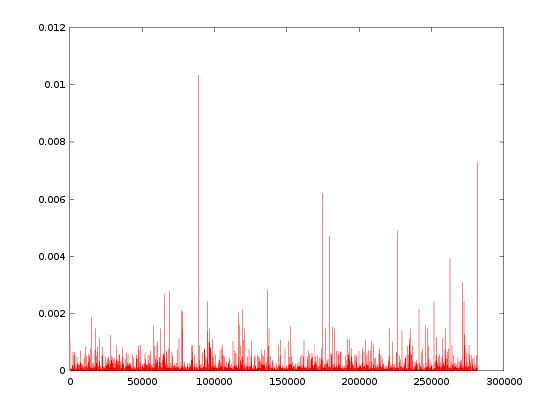
\includegraphics[width=.70\textwidth]{figs/confronto_tempi_corr_1.jpg}} \\
\subfloat[][\emph{alpha=0.11}]
{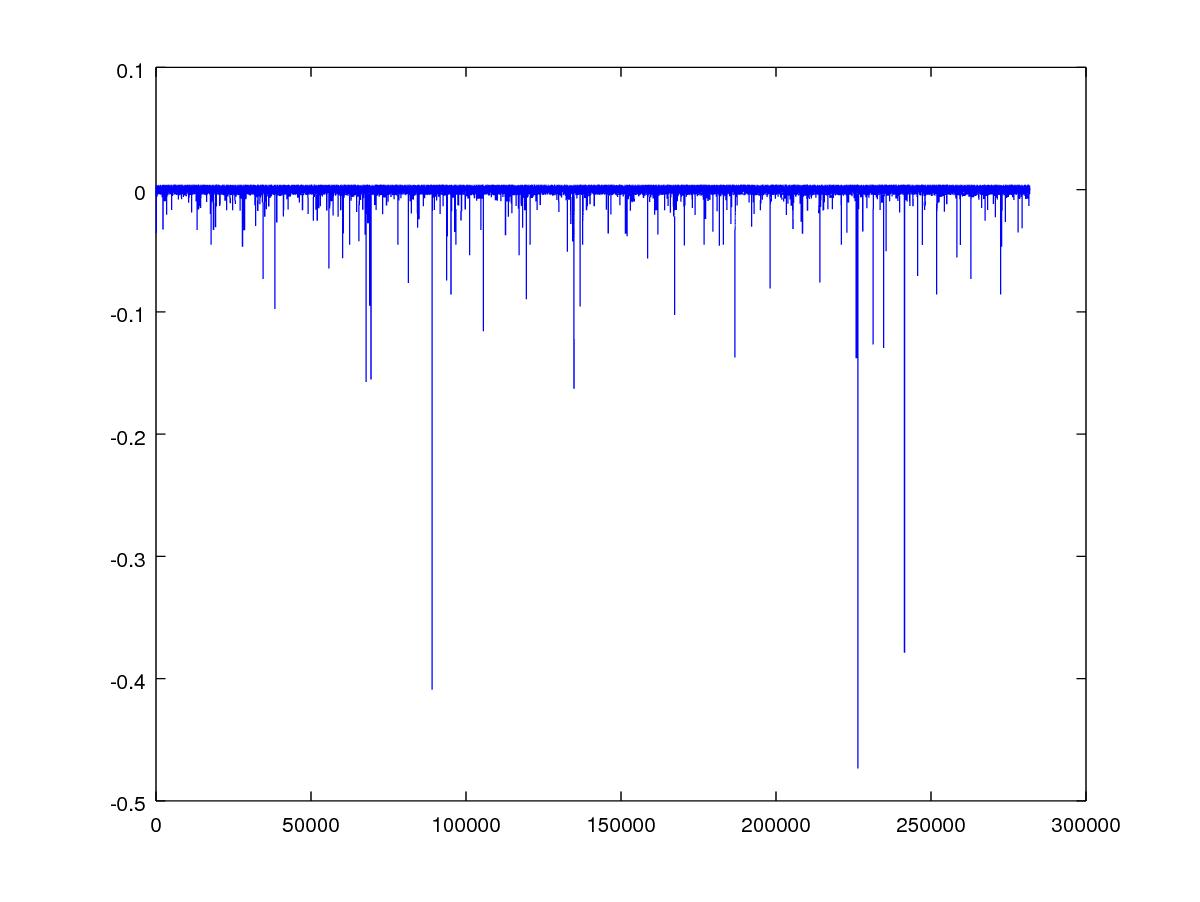
\includegraphics[width=.70\textwidth]{figs/confronto_tempi_corr_2.jpg}} \quad
\caption{Immagini ottenute da \emph{confronto\_tempi}.}
\end{figure}
\newpage
Da queste immagini si può vedere come le componenti dei vettori differenza siano tutte molto piccole, inferiori in valore
assoluto a 0.012 nel caso \emph{alpha = 0.15} ed inferiori a 0.5 nel caso \emph{alpha = 0.11}. Le soluzioni ottenute con i due metodi
sono dunque molto vicine tra loro.

% ##########################################  A QUI #######################################

\chapter{Lezione VI, 17 Marzo 2017}
\section{Esercizio 1}
La funzione \emph{Hiterate\_HITS} è:
\begin{lstlisting}[frame=trBL]
function [h, a]=Iterate_HITS(A)
% A matrice di adiacenza di un grafo
% h e a punteggi di Hub e autority

iter=3000;
epsilon=10^-16;

h0=ones(size(A,2),1);
a0=ones(size(A,2),1);
h=A*a0;
a=a0;
B=A';
i=0;
while (norm(h-h0)>epsilon || norm(a-a0)>epsilon) & i<iter
    h0=h;
    a0=a;
    a=B* h0;
    h=A*a;
    h=h/norm(h, 2);
    a=a/norm(a, 2);
    i=i+1;
end
\end{lstlisting}
Confontiamo i risultati con quelli ottenuti tramite il comando \emph{eigs}:
\begin{lstlisting}[frame=lines]
>>load('QMATRIX.mat')
>>[h,a]=Iterate_HITS(Q)
h =

   0.00000
   0.00000
   0.52573
   0.00000
   0.00000
   0.00000
   0.42533
   0.42533
   0.42533
   0.42533


a =

   0.97325
   0.00000
   0.00000
   0.22975
   0.00000
   0.00000
   0.00000
   0.00000
   0.00000
   0.00000
>> [A,~]=eigs(Q'*Q,1,'LM')

A =

   -0.9732
    0.0000
    0.0000
   -0.2298
    0.0000
    0.0000
    0.0000
    0.0000
    0.0000
    0.0000

>> [H,~]=eigs(Q*Q',1,'LM')

H =

    0.0000
   -0.0000
   -0.5257
   -0.0000
    0.0000
   -0.0000
   -0.4253
   -0.4253
   -0.4253
   -0.4253
\end{lstlisting}
\newpage
\section{Esercizio 2}
La funzione \emph{rank\_compare} è:
\begin{lstlisting}[frame=trBL]
function [top_idx, pr_idx, auth_idx]=rank_compare(A, n)}
% A matrice di adiacenza di un grafo
% n: intero positivo
% top_idx: vettore di indici dei primi n nodi ordinati in base
% a somma di indegree e outdegree
% pr_idx: vettore di indici dei primi n nodi ordinati
% in base a pagerank
% auth_idx:vettore di indici dei primi n nodi ordinati in base
% al punteggio di authority

indegree = sum(A);
outdegree = sum(A');
sumdegree = indegree + outdegree;
[B,I]=sort(sumdegree,'descend'); %ordino il vettore sumdegree
top_idx=I(1:n);
C=A(top_idx,top_idx); %riordino a secondo 
                      %le prime n componenti di I
pr=pagerank(C,0.15);
[Bpr,Ipr]=sort(pr,'descend');
pr_idx=top_idx(Ipr);
[a,h]=Iterate_HITS(C);
[Bh,Ih]=sort(h,'descend');
auth_idx=top_idx(Ih);
\end{lstlisting}
Mostriamo le prime dieci componenti dei 3 vettori di ranking:
\begin{lstlisting}[frame=trBL]
>>A=spconvert(stanford_web);
>>[top_idx, pr_idx, auth_idx]=rank_compare(A,10);
>>B=[top_idx; pr_idx; auth_idx]'

B=

   226411   241454    81435
   234704   245659   214128
   105607   167295   198090
   241454   234704   105607
   167295   226411   226411
    38342    38342   234704
    81435    81435   167295
   214128   214128    38342
   198090   198090   245659
   245659   105607   241454
\end{lstlisting}

\section{Esercizio 3}
Per confrontare l'ordinamento indotto da ac con quelli ottenuti con le altre strategie, modifichiamo leggermente la function \emph{rank\_compare} in modo che ci restituisca la matrice ordinata e troncata; per fare questo basta aggiungere nella dichiarazione di funzione, tra le variabili di output, la variabile C:
\begin{lstlisting}[frame=trbl]
function [top_idx, pr_idx, auth_idx,C]=rank_compare(A, n)
\end{lstlisting}
Creiamo quindi la function \emph{centrality.m}:
\begin{lstlisting}[frame = trBL]
function [hc, ac]=centrality(A)
% A : matrice di adiacenza
% hc: misura di centralita' come hub
% ac: misura di centralita' come authority

[n,m]=size(A);
B=[zeros(n,n), A; A', zeros(n,n)];
E=expm(B);
hc=diag(E(1:n,1:n));
ac=diag(E(n+1:2*n,n+1:2*n));
\end{lstlisting}
Calcoliamo la matrice C e i vari ordinamenti di rank\_compare con il comando:
\begin{lstlisting}[frame=lines]
>>A=spconvert(stanford_web);
>>[top_idx,pr_idx,auth_idx,C]=rank_compare(A,1000);
\end{lstlisting}
Procediamo calcolando ac con centrality, calcolandone inoltre l'ordinamento
\begin{lstlisting}[frame=lines]
>>[ac,~]=centrality(C);
>>[~,ordac]=sort(ac,'descend');
\end{lstlisting}
Quindi facciamo il plot di questi 4 vettori:
\begin{lstlisting}[frame=lines]
>>figure(1)
>>plot(ordac)
>>figure(2)
>>plot(top_idx)
>>figure(3)
>>plot(pr_idx)
>>figure(4)
>>plot(auth_idx)
\end{lstlisting}
Ottenendo quindi le seguenti immagini:
\begin{figure}[h!]
\centering
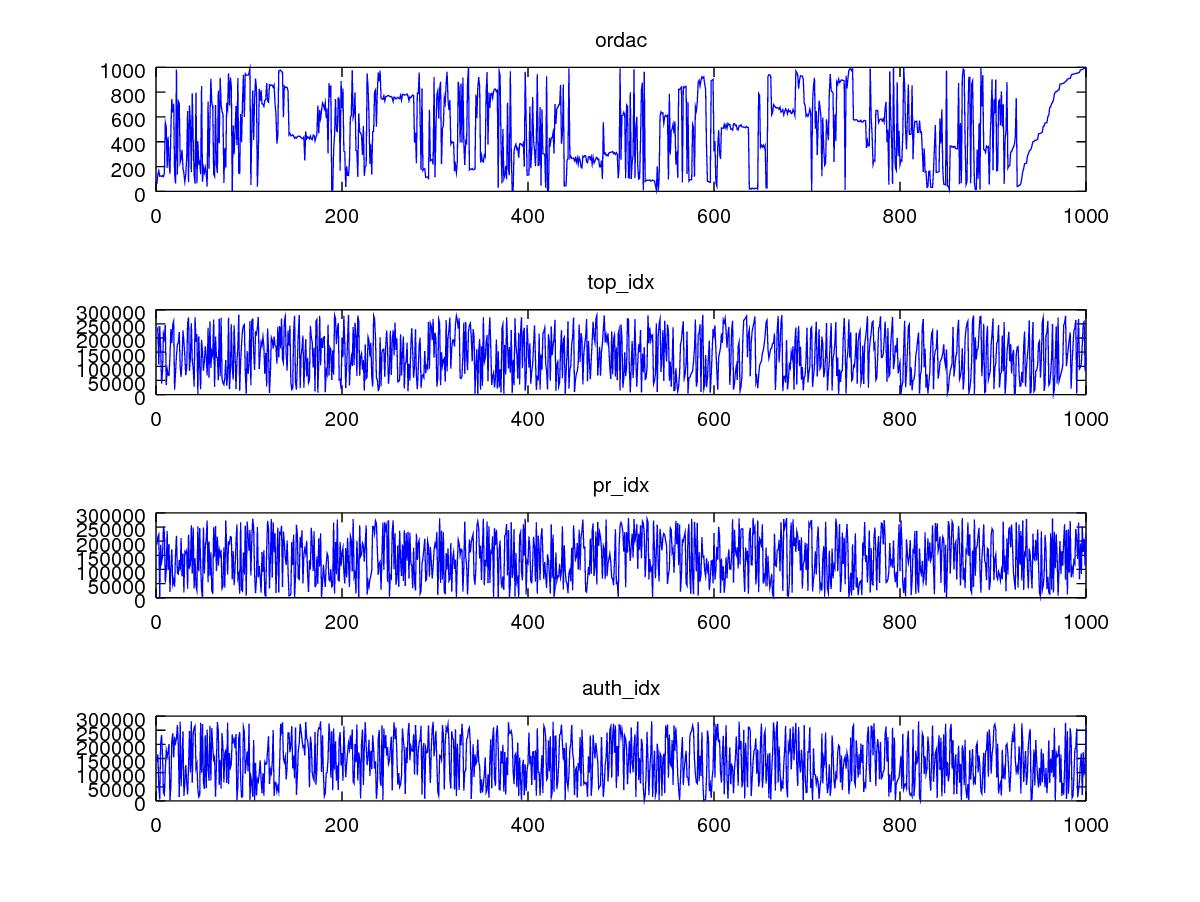
\includegraphics[width=\textwidth]{figs/rank_compare.jpg}
\caption{Immagini degli ordinamenti ac, top, pr, auth.}
\end{figure}

%\begin{figure}[h!]
%\centering
%\subfloat[][\emph{ordac}]
%{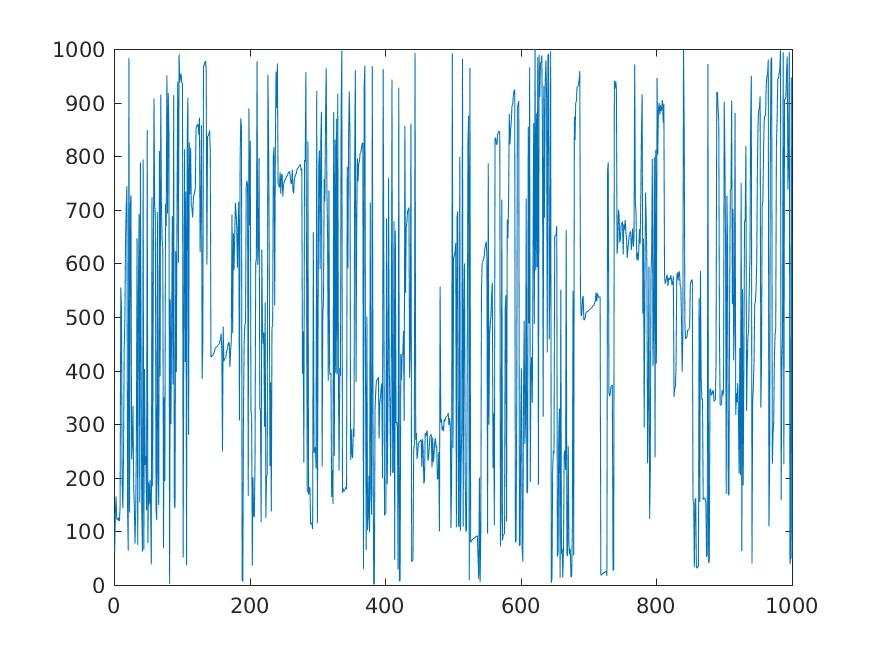
\includegraphics[width=.65\textwidth]{figs/ordac.jpg}} \\
%\subfloat[][\emph{top\_idx}]
%{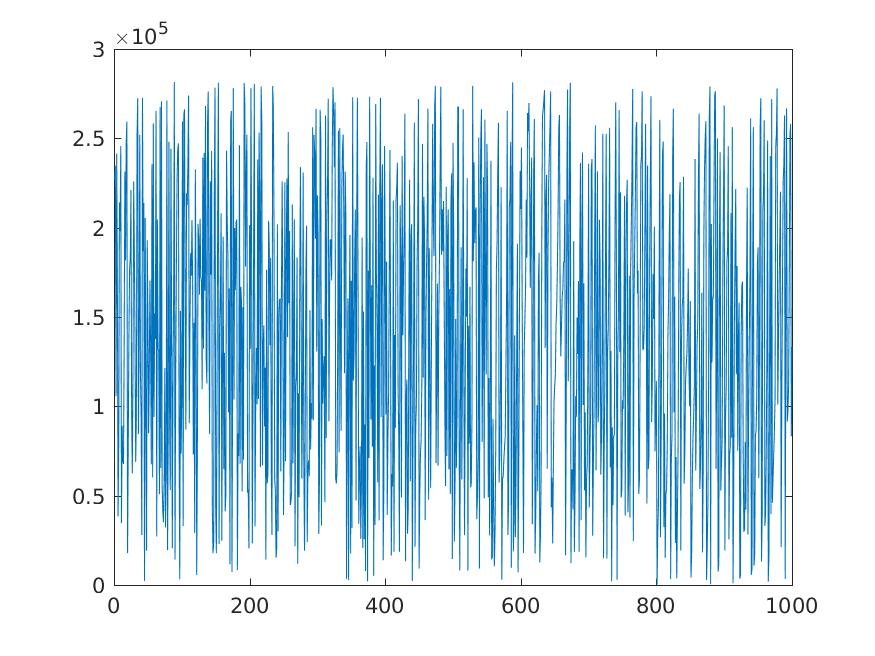
\includegraphics[width=.65\textwidth]{figs/top_idx.jpg}} \\
%\subfloat[][\emph{pr\_idx}]
%{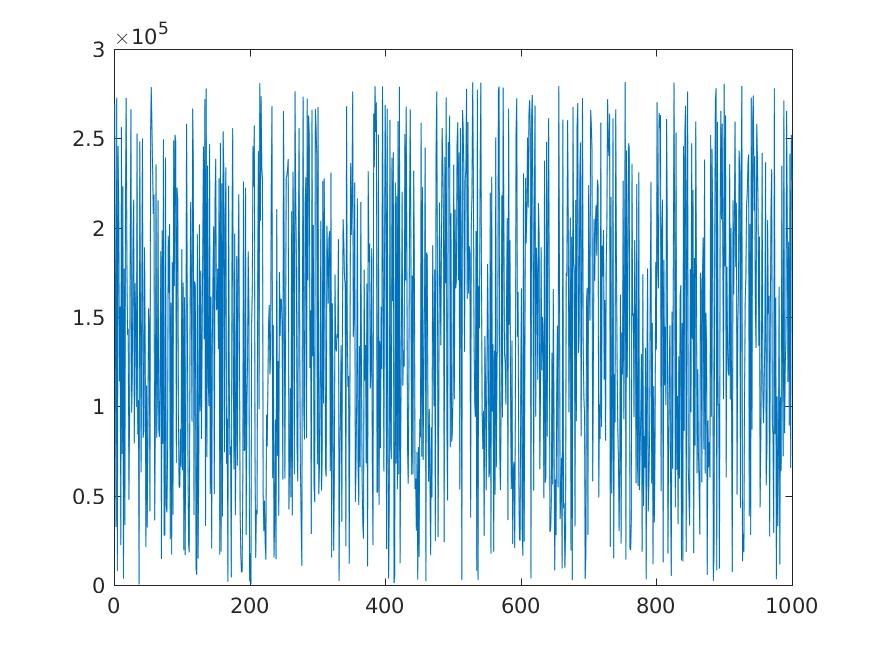
\includegraphics[width=.65\textwidth]{figs/pr_idx.jpg}} \\
%\subfloat[][\emph{auth\_idx}]
%{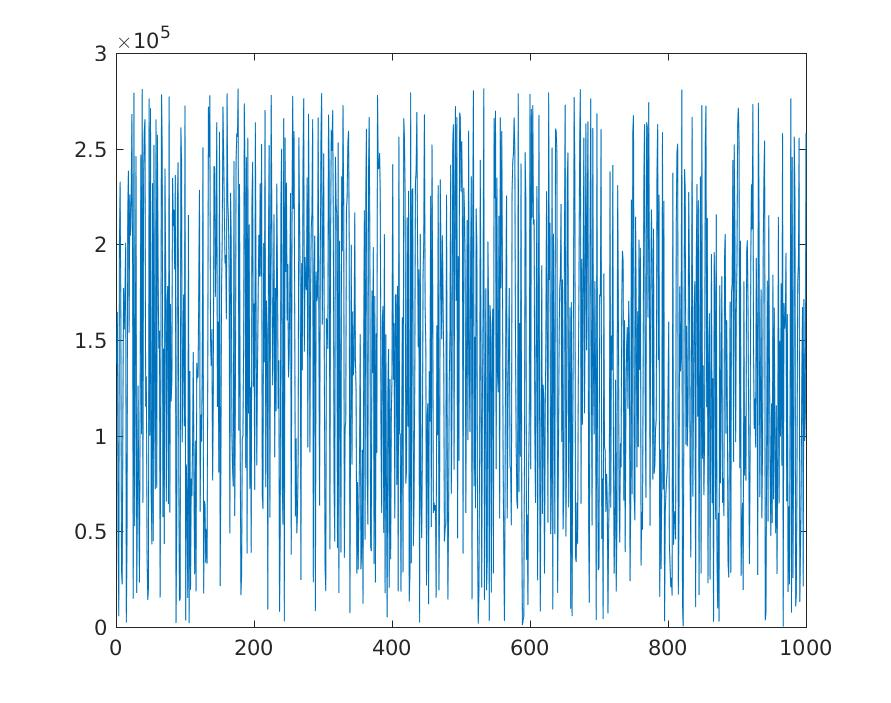
\includegraphics[width=.65\textwidth]{figs/auth_idx.jpg}}
%\caption{Immagini degli ordinamenti ac, top, pr, auth.}
%\end{figure}

\chapter{Lezione VII, 22 Marzo 2017}
\section{Esercizio 1}
La funzione \emph{similarity} è:
\begin{lstlisting}[frame=trBL]
function [S_user, S_items]=similarity(A)
% A; matrice dei rating utenti-items
% S_user: matrice di similarita' (misura del coseno) 
% tra ogni coppia di utenti di A
% S_items; matrice di similarita' (misura del coseno) 
%tra ogni coppia di items di A

[m,n]=size(A);
B=A;
S_user=zeros(m,m);
S_items=zeros(n,n);
%costruiamo la matrice S_user
for p=1:m
    B(p,:)=B(p,:)/norm(B(p,:));
end
for i=1:m
    for j=1:m
        S_user(i,j)=B(i,:)*B(j,:)';
    end
end
%costruiamo la matrice S_items
B=A;
for q=1:n
    B(:,q)=B(:,q)/norm(B(:,q));
end
for i=1:n
    for j=1:n
        S_items(i,j)=C(:,i)'*C(:,j);
    end
end
\end{lstlisting}
\newpage
\section{Esercizio 2}
La funzione \emph{recommend} è:
\begin{lstlisting}[frame=trBL]
function [items_list]=recommend(A, user)
% A: matrice dei rating utenti-items
% user: indice di un utente
% items_list: insieme di indici di item da raccomandare a user

[m,n]=size(A);
[S_user,~]=similarity(A);
items_list=zeros(1,n);
[~,I]=sort(S_user(user,:),'descend');
i_max=I(2);
for j=1:n
    if ((A(user,j)==0) & ((A(i_max,j)==4) || (A(i_max,j)==5)))
        items_list(j)=1;
    end
end
\end{lstlisting}
\section{Esercizio 3}
La funzione \emph{accuracy} è:
\begin{lstlisting}[frame=trBL]
function [p, r]=accuracy(B, item_list, user)
% B: matrice user-items (test-set)
% item_list: insieme di indici
% user: identificativo di un utente
% p: valore di precision
% r: valore di relall

[n,m]=size(B);
tp=0;
fp=0;
fn=0;
for j=1:m
    if (items_list(j)>0) & (B(user,j)>=4)
        tp=tp+1;
    elseif (items_list(j)>0) & (0<B(user,j)<4)
        fp=fp+1;
    elseif (items_list(j)==0) & (B(user,j)>=4)
        fn=fn+1;
    end
end
p=tp/(tp+fp);
r=tp/(tp+fn);
\end{lstlisting}
Per calcolare l'insieme di item da raccomandare per ogni utente nel Test-set usiamo la funzione \emph{accuracy\_2}:
\newpage
\begin{lstlisting}[frame=trBL]
function [p,r,p_media,r_media]=accuracy_2(A,B)
j=0;
[m,~]=size(B);
for i=1:m
    if norm(B(i,:))~=0
        j=j+1;
        items_list=recommend(A,i);
        [p(j),r(j)]=accuracy(B,items_list,i);
    end
end

p_media=sum(p)/j;
r_media=sum(r)/j;
\end{lstlisting}
\section{Esercizio 4}
\subsection{\textbf{Parte 1}}
La funzione \emph{transform} è:
\begin{lstlisting}[frame=trBL]
function [A_mean]=transform(A)}
% A: matrice user-items
% A_mean: marice user_items

[m,n]=size(A);
A_mean=A;
for i=1:m
    mean=mean(A(i,:));
    for j=1:n
        if A_mean(i,j)==0
            A_mean(i,j)=mean;
        end
    end
end
\end{lstlisting}
\newpage
\subsection{\textbf{Parte 2}}
La funzione \emph{pure\_svd} è:
\begin{lstlisting}[frame=trBL]
function [C]=pure_svd(A, k)}
% A: matrice user-items
% C: matrice user_items

[m,n]=size(A);
A_mean=transform(A);
X=A;
C=zeros(m,n);
%SVD di rango k di A_mean
[S,V,D]=svds(A_mean,k);
M=S*V*D';
for i=1:m
    for j=1:n
        if X(i,j)==0
            X(i,j)=M(i,j);
        end
        if X(i,j)<=0
            C(i,j)=0;
        elseif 0<X(i,j)<5
            C(i,j)=round(X(i,j));
        else
            C(i,j)=5;
        end
    end
end
\end{lstlisting}
\subsection{\textbf{Parte 3}}
La funzione \emph{recommend\_svd} è:
\begin{lstlisting}[frame=trBL]
function [U]=recommend_svd(A,C)
% A: matrice user-item
% C: matrice user-item ottenuta con la funzione pure_svd
% U: matrice user-item binaria

[m,n]=size(A);
U=zeros(m,n);
for i=1:m
    for j=1:n
        if (A(i,j)==0) & (C(i,j)>=4)
            U(i,j)=1;
        end
    end
end
\end{lstlisting}
Per calcolare i valori medi di precision e recall su tutti gli utenti del Test-set usiamo la seguente funzione:
\newpage
\begin{lstlisting}[frame=trBL]
function [p,r,p_media,r_media]=accuracy_3(A,B,k)
j=0;
[n,m]=size(B);
C=pure_svd(A,k);
U=recommend_svd(A,C);
for i=1:n
    if norm(B(i,:))~=0
        j=j+1;
        [p(j),r(j)]=accuracy(B,U(i,:),i);
    end
end
p_media=sum(p)/j;
r_media=sum(r)/j;
\end{lstlisting}
\end{document}
